\documentclass[tikz,border=2pt]{standalone}
\usepackage{amsmath,amssymb}
\usepackage{pgfplots}
\pgfplotsset{compat=1.18}
\usetikzlibrary{arrows.meta}
\begin{document}
% Exponential order X <=_e Y for X = 1 and Y in {0,2} with probability 1/2 each:
% M_X(alpha) = e^alpha lies below M_Y(alpha) = (1+e^{2 alpha})/2 for every alpha > 0; both equal 1 at alpha = 0.
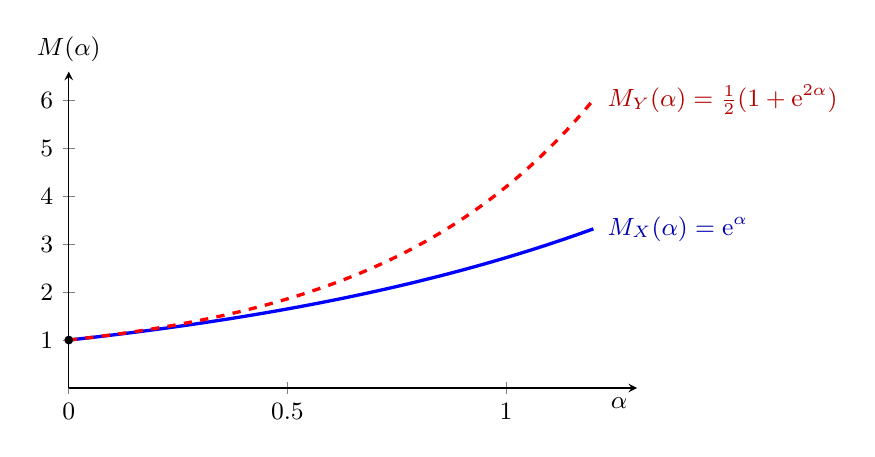
\begin{tikzpicture}[font=\small, >={Latex[length=2mm]}]
  \begin{axis}[
    axis lines=left, xmin=0, xmax=1.3, ymin=0, ymax=6.6,
    xtick={0,0.5,1}, ytick={1,2,3,4,5,6},
    xlabel={$\alpha$}, ylabel={$M(\alpha)$},
    xlabel style={at={(axis description cs:1,0)}, anchor=north east},
    ylabel style={rotate=-90, at={(axis description cs:0,1)}, anchor=south},
    width=8.8cm, height=5.6cm, clip=false
    ]
    \addplot[blue, very thick, domain=0:1.2, samples=60] {exp(x)};
    \addplot[red, very thick, dashed, domain=0:1.2, samples=60] {(1+exp(2*x))/2};
    \fill[black] (axis cs:0,1) circle (1.6pt);
    \node[blue!70!black, anchor=west] at (axis cs:1.21,3.32) {$M_X(\alpha)=\mathrm{e}^{\alpha}$};
    \node[red!70!black, anchor=west] at (axis cs:1.21,6.01) {$M_Y(\alpha)=\tfrac{1}{2}(1+\mathrm{e}^{2\alpha})$};
  \end{axis}
\end{tikzpicture}
\end{document}
